% !TeX root = ./main.tex
\documentclass[main]{subfiles}
\begin{document}
\part*{Общая топология}
\chapter{Метрические пространства}
\section{Метрические пространства}
\begin{definition}
    $M$ -- множество. $M$ вместе с $\rho: M \times M \to \R$ называется
    метрическим пространством, если:
    \begin{enumerate}
        \item $\forall x,y \ \rho(x,y) \ge 0$ и $\rho(x,y) = 0 \Leftrightarrow x=y$
        \item $\forall x,y \ \rho(x,y) = \rho(y,x)$
        \item Неравенство треугольника: $\rho(x,z) \le \rho(x,y) + \rho(y,z)$
    \end{enumerate}
    $(M, \rho)$ -- метрическое пространство, $\rho$ -- метрика на $M$.
\end{definition}
\begin{example}
    $M$ -- множество домов в городе. $\rho(x,y)$ -- минимальное время,
    за которое можно добраться от $x$ до $y$.
    (1 свойство очевидно, 2 свойство выполняется при симметричности дорог, 3 очевидно)
\end{example}
\begin{example}
    Расстояние на плоскости.
    \begin{gather*}
        \R^2 = \{(x,y):x,y \in \R\}\\
        \rho_1((x_1, y_1), (x_2, y_2)) \coloneqq |x_1 - x_2| + |y_1 - y_2|\\
        \rho_2((x_1, y_1), (x_2, y_2)) \coloneqq \sqrt{(x_1 - x_2)^2 + (y_1 - y_2)^2}\\
        \rho_k((x_1, y_1), (x_2, y_2)) \coloneqq \left(|x_1 - x_2|^k + |y_1 - y_2|^k\right)^{1/k}\\
        k \to \infty: \rho_\infty((x_1, y_1), (x_2, y_2)) \coloneqq \max\{|x_1 - x_2|; |y_1 - y_2|\}
    \end{gather*}
    Если перейти к $\R^n$, то
    \[\rho_k((x_1,x_2,..., x_n); (y_1, y_2,...,y_n)) = \left(\sum_{i=1}^n |x_i-y_i|^k\right)^{1/k}\]
\end{example}
\begin{gather*}
    \begin{multlined}
        \left(|\underbrace{x_1-x_3}_{a_1+b_1}|^k + |\underbrace{y_1-y_3}_{a_2+b_2}|^k\right)^{1/k} \le
        \left(|\underbrace{x_1-x_2}_{a_1}|^k + |\underbrace{y_1-y_2}_{a_2}|^k\right)^{1/k}+\\
        \left(|\underbrace{x_2-x_3}_{b_1}|^k + |\underbrace{y_2-y_3}_{b_2}|^k\right)^{1/k}
    \end{multlined}\\
    \left(\sum|a_i+b_i|^k\right)^{1/k} \le \left(|a_1|^k + |a_2|^k\right)^{1/k} + \left(|b_1|^k + |b_2|^k\right)^{1/k}
\end{gather*}
Неравенство Йенсена (к чему это?)

\begin{definition}
    $B(x_0, r)\coloneqq\{x\in M : \rho(x,x_0) < r\}$ -- шар с центром в точке $x_0$ и радиусом $r$.
\end{definition}

Нарисуем $B((0,0);1)$ в $\rho_1, \rho_2, \rho_\infty.$

\begin{center}
    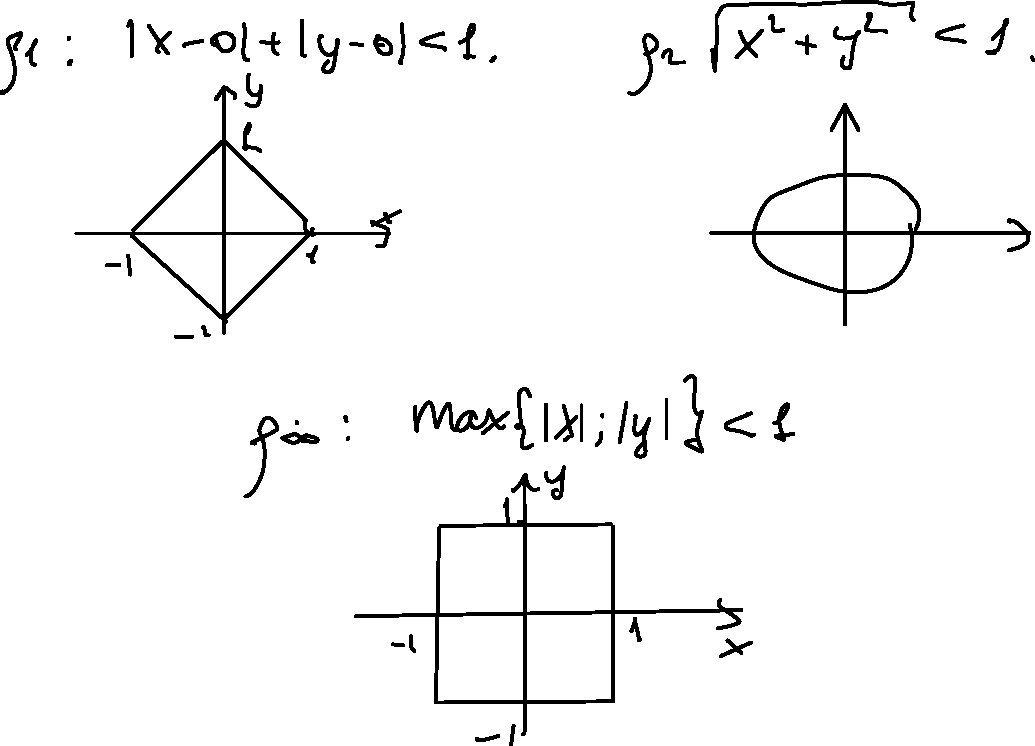
\includegraphics[width=\textwidth]{ball_examples.pdf}
\end{center}

\begin{minipage}{0.45\textwidth}
    $\rho_1$ называется манхэттенской метрикой.
\end{minipage}
\begin{minipage}{0.45\textwidth}
    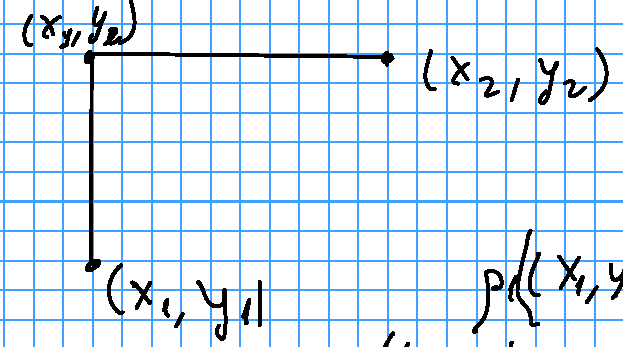
\includegraphics[width=\textwidth]{manhattan_distance.pdf}
\end{minipage}
\begin{gather*}
    \rho_1((x_1, y_1), (x_2, y_2)) = |x_1 - x_2| + |y_1 - y_2|\\
    \rho_1((x_1, y_1), (x_1, y_2)) = |y_1 - y_2|\\
    \rho_1((x_1, y_2), (x_2, y_2)) = |x_1 - x_2|
\end{gather*}

\begin{example}
    $M$ --  пространство <<некоторых>>\footnote{<<некоторых>> -- обладающих естественными свойствами, какими именно -- зависит от функци}
    функций. Функции определены на $X\subset \R$.
    \[\rho_1(f,g) \coloneqq \int_X |f(x)-g(x)| dx\]
    Есть проблемы: если $f(x)=g(x)$ всюду, кроме 1 точки, то $\rho_1(f,g)=0$.

    1 и 2 свойство очевидны. Третье:
    \[\int_X |f-h| dx \le \int_X|f-g|dx + \int_X |g-h|dx\]
    Аналогично определяются другие метрики, например:
    \begin{gather*}
        \rho_2(f,g) = \left(\int_X |f(x)-g(x)|^2 dx\right)^{1/2}\\
        \rho_k(f,g) = \left(\int_X |f(x)-g(x)|^k dx\right)^{1/k}\\
        \rho_\infty(f,g) = \sup_{x\in X} |f(x)-g(x)|
    \end{gather*}

    Естественные свойства:
    \begin{gather*}
        \rho_2: \int_X |f(x)|^2 dx < \infty
    \end{gather*}
\end{example}

\begin{definition}
    $(M, \rho)$ -- метрическое пространство. $\{x_n\}^\infty_{n=1} \subset M$ -- последовательность.
    Говорим, что $\lim_{n\to\infty} x_n = x_0$, если
    \[\forall \epsilon>0 \ \exists N(\epsilon): \forall n > N \ \rho(x_n; x_0) < \epsilon\]
\end{definition}

В частности, в пространстве функций с разными метриками бывают разные пределы последовательностей функций.
\[f_n(x) \to f_0(x) \text{ по метрике } \rho_1\]
Аналогично для других метрик.

\[f_n(x) \to f_0(x) \text{ по метрике } \rho_\infty\]
называется равномерной сходимостью. $f_n \rightrightarrows f_0$:
\[f_n(x) \rightrightarrows f_0(x) \Leftrightarrow \lim \sup_X |f_n(x) - f_0(x)|\]

\begin{example}
    Дискретное метрическое пространство. $M$ -- любое множество.
    \[\rho(x,y) = \begin{cases}
            1 & x \neq y \\
            0 & x =y
        \end{cases}\]
    дискретная метрика.
\end{example}

\begin{example}
    На самом деле дискретная метрика -- это обобщение $\rho(x,y) \ge \epsilon >0$.
    $\epsilon$ не зависит от $x$ или $y$.
\end{example}

\begin{example}
    $M$ -- множество строк длины $n$. $\rho(x,y)$ -- количество символов, где эти
    строки отличаются
\end{example}

\begin{example}
    Задача: есть код из $N$ бит. Можем переслать, но возникнет не более $k$ ошибок.
    Сколько бит надо переслать, чтобы эти ошибки можно было исправить?

    Решать не будем, переформулируем на язык метрических пространств.

    $(M,\rho)$. $M$ состоит из строк, каждая из $N+k$ двоичных символов.
    Хотим выбрать $\{x_1, x_2,..., x_{2^N}\} \subset M: \rho(x_i, x_j) > 2k$.
    $l \to \min$.

    $x_i$ -- строки из $N+l$ символов.
    \begin{gather*}
        x_i = a_{i1}a_{i2}...a_{iN+l}\\
        x_j = b_{i1}b_{i2}...b_{iN+l}
    \end{gather*}
\end{example}

\section{Расположение точки относительно множества}
\begin{center}
    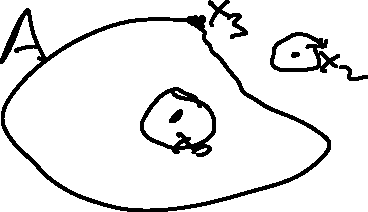
\includegraphics[width=0.5\textwidth]{dot_placement.pdf}
\end{center}
\begin{theorem}[Жордана]
    Любая замкнутая непересекающаяся кривая на плоскости делит
    плоскость на две части; равно одна из частей не ограничена.
\end{theorem}
\begin{proof}
    Доказать невероятно сложно.
\end{proof}

\subsection{Кривая Пеано}
\[f:[0,1] \to [-1,1] \times [-1,1]\]
\begin{center}
    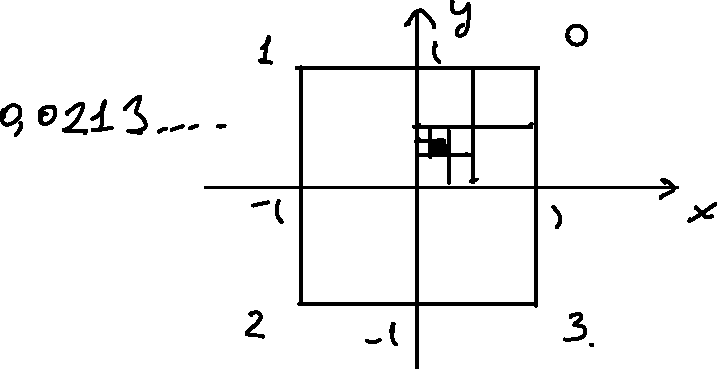
\includegraphics[width=0.8\textwidth]{peano_curve.pdf}
\end{center}
Разложим $a \in [0,1]$ в четверичную систему счисления: $a = 0.a_1 a_2 a_3 a_4 ...$.
Если $a_1 = 0$, то идем в I квадрант. Разбиваем его на 4 части.
Далее, если $a_2=2$, то идем в III квадрант, и так далее.

То есть, сопоставляем числу последовательность квадратов.
Эта последовательность квадратов сходится к одной точке.

По теореме о вложенных отрезках, пересечение квадратов не пусто.
Но это пересечение не может состоять более чем из одной точки.

\begin{minipage}{0.45\textwidth}
    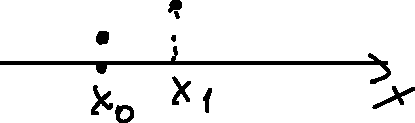
\includegraphics[width=\textwidth]{peano_curve_one_point.pdf}
\end{minipage}
\begin{minipage}{0.45\textwidth}
    Подберем $N$:
    \begin{gather*}
        |x_0 - x_1| > 2^{-N}\\
        2^N > \frac{1}{|x_0 - x_1|}
    \end{gather*}
\end{minipage}

Кривая Пеано сопоставляет точке $a = 0.a_1 a_2 a_3...$ единственную
существующую точку, содержащуюся в пересечении всех соответствующих квадратов

Почему эта кривая непрерывна?
\begin{gather*}
    |a-b|<\delta\\
    a = 0. a_1 a_2 a_3 ... \qquad b = 0. b_1 b_2 b_3 ...
\end{gather*}

Это значит, что либо
\[a_1 = b_1, a_2 = b_2, ..., a_k = b_k\]
либо
\[a_1 = b_1,..., a_{l-1} = b_{l-1} \text{ и } b_l= a_{l+1} = ... = a_k =3,  b_{l+1} = ... = b_k =0\]
$k$ достаточно большое число
\begin{center}
    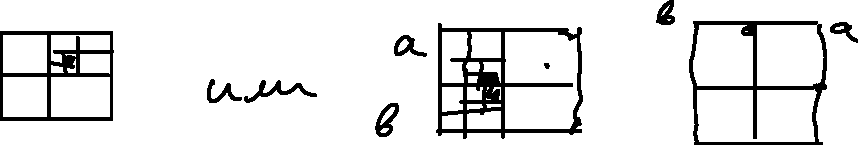
\includegraphics[width=0.8\textwidth]{peano_curve_continuity.pdf}
\end{center}

Строится кривая, чтобы она была непрерывна. Такая кривая полностью заметает квадрат.

Существуют кривые, такие что их образ покрывают квадрат.

\subsection{Определения}
\begin{definition}
    $(M, \rho)$ -- метрическое пространство. $A \subset M, x_0 \in M (x_0 \in A \text{ или } x_0 \not\in A)$.

    $B(x_0, \epsilon) \coloneqq \{x: \rho(x, x_0) < \epsilon\}$ -- шар с центром в $x_0$ и радиусом $\epsilon$.

    $x_0$ называется внутренней точкой  для $A$, если $\exists \delta>0 : B(x_0, \delta) \subset A$.

    $x_0$ называется внешней точкой  для $A$, если $\exists \delta>0 : B(x_0, \delta) \cap A = \varnothing$.

    В противном случае точка называется граничной.
    А именно, $x_0$ -- граничная, если
    $\forall \delta >0 \ B(x_0, \delta) \not\subset A \text{ и }
        B(x_0, \delta) \cap A \neq \varnothing$, то есть
    $\exists x_1 \in  B(x_0, \delta) \cap A \text{ и }
        \exists x_2 \in B(x_0, \delta) \setminus A$.
\end{definition}

\begin{definition}
    Множество внутренних точек $A$ называется внутренностью $A: \Int A$.

    Множество внешних точек $A$ называется внешностью $A: \Ex A$.

    Множество граничных точек $A$ называется границей $A: \partial A$ или $\operatorname{Fr}A$
\end{definition}
\begin{remark}
    Эти множества не пересекаются. В объединении -- множество $M$.
\end{remark}

\begin{definition}
    Замыкание $A: \Cl A = \Int A \cup \partial A$
    или $\Cl A = M \setminus \Ex A$
\end{definition}

\begin{definition}
    $U \subset M$. $U$ называется открытым, если $U= \Int U$.
    Или $\forall x_0 \in U \exists \epsilon > 0: B(x_0, \epsilon) \subset U$
\end{definition}

\begin{theorem}[Cвойства открытых множеств]
    \

    \begin{enumerate}
        \item $\{U_i\}_{i \in I}$ -- семейство открытых множеств, тогда $\bigcup_{i \in I} U_i$ открыто.
        \item $U_1, U_2, ..., U_n$ -- открытые множества, тогда $\bigcap_{i=1}^n U_i$  открыто.
        \item $\varnothing, M$ открыто
    \end{enumerate}
\end{theorem}
\begin{proof}
    \

    \begin{enumerate}
        \item Возьмем
              $x_0 \in \bigcup_{i \in I} U_i \implies \exists i_0: x_0 \in U_{i_0}$.
              Пусть $U_{i_0}$ открыто, тогда
              $\exists \delta > 0: B(x_0, \delta) \subset U_{i_0} \subset \bigcup_{i \in I} U_i$.
              Значит, $\bigcup_{i \in I} U_i$ открыто
        \item Рассмотрим $\forall x_0 \in \bigcap_{i=1}^n U_i \implies \forall i: x_0 \in U_i$.
              Значит $\exists \delta_i > 0: B(x_0, \delta_i) \subset U_i$.
              Возьмем $\delta \coloneqq \min \{\delta_1, \delta_2, ..., \delta_n\} > 0$.
              $B(x_0, \delta) \subset B(x_0, \delta_i) \subset U_i\ \forall i$.
              Раз выполнено для любого $i$, значит $B(x_0, \delta) \subset \bigcap_{i=1}^n U_i$
        \item Очевидно \qedhere
    \end{enumerate}
\end{proof}

\begin{definition}
    $F \subset M$, $F$ называется замкнутым множеством, если $M \setminus F$ открыто.
\end{definition}
\begin{theorem}[Свойства замкнутых множеств]
    \

    \begin{enumerate}
        \item $\{F_i\}_{i \in I}$ -- семейство замкнутых множеств, значит $\bigcap_{i \in I} F_i$ замкнуто.
        \item $F_1, F_2, ..., F_n$ -- замкнутые множества, значит $\bigcup_{i=1}^n F_i$ замкнуто.
        \item $\varnothing, M$ замкнуты
    \end{enumerate}
\end{theorem}
\begin{proof}
    Упражнение.

    Hint: $U_i \coloneqq M \setminus F_i$. $U_i$ открытое $\Leftrightarrow F_i$ замкнутое.
    По формулам де Моргана: $M \setminus (F_1 \cup F_2) = (M\setminus F_1) \cap (M \setminus F_2)$ и т.д..
\end{proof}

\begin{lemma}\label{spaces:1}
    $B(x_0, \delta)$ -- открытое множество.
\end{lemma}
\begin{proof}
    \

    \begin{minipage}{0.45\textwidth}
        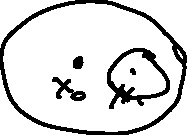
\includegraphics[width=0.7\textwidth]{open_ball.pdf}
    \end{minipage}
    \begin{minipage}{0.45\textwidth}\raggedright
        Пусть $x_1 \in B(x_0, \delta)$,  $\rho(x_0, x_1) = \epsilon < \delta$.

        Если взять $r \coloneqq \delta - \epsilon$, то $B(x_1, r) \subset B(x_0, \delta)$.
        Почему так?
    \end{minipage}

    Допустим $x_2 \in B(x_1, r)$, то есть $\rho(x_1, x_2) < r = \delta - \epsilon$.
    Но допустим $x_2 \not\in B(x_0, \delta)$, то есть $\rho(x_0, x_2) \ge \delta$.

    $\underbrace{\rho(x_0, x_2)}_{\ge \delta} \le \underbrace{\rho(x_0, x_1)}_{= \epsilon} + \underbrace{\rho(x_1, x_2)}_{< \delta- \epsilon}$ -- противоречие.
\end{proof}


\begin{theorem}
    $M$ -- метрическое пространство; $A \subset M$; Тогда
    \[\Int A = \bigcup_{\substack{U_i \text{ открыто}\\ U_i \subset A}} U_i, \]
    где $U_i$ открыты и $U_i \subset A$
\end{theorem}
\begin{proof}
    $\displaystyle \bigcup_{\substack{U_i \text{ открыто}\\ U_i \subset A}} U_i$ открыто.
    $\Int A$  -- открытое множество по лемме \ref{spaces:1}.

    Если $x_0$ внутренняя точка, а $x_1 \in B(x_0, \delta) \subset A$,
    тогда по лемме $x_1$ -- внутренняя точка $B(x_1, \delta - \rho(x_0, x_1)) \subset B(x_0, \delta) \subset A$,
    значит все точки шара являются внутренними.

    $\Int A = \bigcup_{x_0 \in \Int A} B(x_0, \delta_{x_0})$, где $B(x_0, \delta_{x_0})\subset A$,
    тогда $\Int A$ является открытым множеством.
    Следовательно $\displaystyle \Int A \subset \bigcup_{\substack{U_i \text{ открыто}\\ U_i \subset A}} U_i$.

    С другой стороны, $\displaystyle \Int A \supset \bigcup_{\substack{U_i \text{ открыто}\\ U_i \subset A}} U_i$.
    Возьмем любое $U_i$, т.ч. оно открыто и $U_i \subset A$.
    По определению $\forall x_o \in U_i\ \exists \epsilon > 0\ B(x_0, \epsilon) \subset A$,
    тогда $x_0 \in \Int A$.

    Итого: $\displaystyle \Int A = \bigcup_{\substack{U_i \text{ открыто}\\ U_i \subset A}} U_i$.
\end{proof}

\begin{corollary}
    Следующие определения внутренности равносильны:
    \begin{enumerate}
        \item Множество внутренних точек
        \item $\displaystyle \bigcup_{B(x_0, \delta) \subset A} B(x_0, \delta)$
        \item $\displaystyle \Int A = \bigcup_{\substack{U_i \text{ открыто}\\ U_i \subset A}} U_i$
        \item $\Int A$ -- максимальное открытое подмножество $A$.
    \end{enumerate}
\end{corollary}

\begin{theorem}
    \[\Cl A = \bigcap_{\substack{F \text{ замкнуто} \\ F \supset A}} F\]
\end{theorem}
\begin{proof}
    Упражнение.
\end{proof}

\begin{example}
    $M = \R; A = \Q$. $A$ не открыто и не замкнуто.
    \[\Int A = \varnothing\qquad \Cl A = \R \qquad \partial A = \R\]
    $B(x_0, \epsilon) = (x_0 - \epsilon; x_0 + \epsilon)$.
    В этом (как и в любом другом интервале) есть рациональные и иррациональные числа,
    тогда $x_0 \in \partial \Q \implies \partial \Q = \R$.
\end{example}

\begin{proposition}
    $(M, \rho)$ -- метрическое пространство. $A \subset M \implies \Cl A$ -- это:
    \begin{enumerate}
        \item $\Int A  \cup \partial A = M \setminus \Ex A = M \setminus \Int (M \setminus A)$
        \item $\displaystyle \bigcap_{\substack{Z \text{ замкнуто}\\ Z \supset A}} Z$
        \item Наименьшее замкнутое множество, которое содержит $A$.
    \end{enumerate}
\end{proposition}
\begin{proof}
    $(2) \Leftrightarrow (3)$: наименьшее замкнутое множество, содержащее $A$ входит в пересечение, т.е. пересечение заведомо не больше.
    Пересечение замкнуто как пересечение замкнутых множеств, и оно содержит $A$, значит оно не меньше, чем наименьшее.

    $(1) \Leftrightarrow (2)$: $x_0 \in \Ex A \implies \exists \epsilon >0: B(x_0, \epsilon) \in \Ex A$ ($B$ открыт).
    $M \setminus B(x_0, \epsilon) \supset A$ -- замкнуто.
    Если $\displaystyle x_0 \in \Ex A \implies x_0 \not\in \bigcap_{\substack{Z \text{ замкнуто}\\ Z \supset A}} Z$.
    Если $x_0 \not\in \Ex A$, допустим, что $\displaystyle x_0 \not\in \bigcap_{\substack{Z \text{ замкнуто}\\ Z \supset A}} Z$.
    Значит существует замкнутое $Z_i: x_0 \notin Z_i$, тогда $x_0$ лежит в открытом $M \setminus Z_i$.
    Но $\exists \epsilon>0: B(x_0, \epsilon) \in M \setminus Z \subset M \setminus A \implies x_0 \in \Ex A$.
\end{proof}

\begin{proposition}
    $U$ -- открытое, $Z$ -- замкнутое.
    \begin{gather*}
        U \setminus Z \text{ -- открытое}\\
        Z \setminus U \text{ -- замкнутое}
    \end{gather*}
\end{proposition}
\begin{proof}
    \[U \setminus Z = U \cap (M \setminus Z),\]
    где $U$ и $M \setminus Z$ открытые, значит их пересечение открыто.
    \[Z \setminus U = Z \cap (M \setminus U),\]
    где $Z$ и $M \setminus U$ замкнутые, значит их пересечение замкнуто.
\end{proof}
\begin{corollary}
    $\Cl A$ замкнуто, $\Cl A = M \setminus \Ex A$.

    $\partial A$ замкнуто, $\partial A = \Cl A \setminus \Int A$.
\end{corollary}

\begin{example}
    Канторово множество.

    \begin{center}
        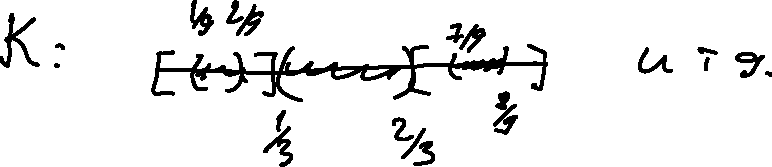
\includegraphics[width=0.7\textwidth]{K.pdf}
    \end{center}

    \[K = \left( \left[0;1\right]
        \setminus \left(\frac{1}{3}; \frac{2}{3}\right) \right)
        \setminus \left( \left(\frac{1}{9}; \frac{2}{9}\right)
        \cup \left(\frac{7}{9}; \frac{8}{9}\right) \right)
        \setminus ...\]
    Мера $K = 0$:
    \[1 - \frac{1}{3} - \frac{2}{9} - \frac{4}{27} - ... =
        1 - \frac{1}{3} \left(1 + \frac{2}{3} + \frac{4}{9} + ...\right) =
        1 - \frac{1}{3} \cdot \frac{1}{1- (2/3)} =
        1 - \frac{1}{3} \cdot 3 = 0\]
    $K$ несчетно. $K = \{0.a_1 a_2 a_3 ...: a_i = \{0, 2\}\}$ в троичной системе.

    $K$ равномощно множеству двоичных бесконечных последовательностей.
    $K$ замкнутое множество.
\end{example}

\begin{theorem}
    $(M, \rho_1)$ и $(M, \rho_2)$ -- два метрических пространства на $M$.
    Пусть существует $C > 0: \forall x,y$
    \[\rho_1 (x,y) \le C \rho_2(x,y)\]
    Тогда, если множество $U$ открыто в $(M, \rho_1)$,
    то $U$ открыто и в $(M, \rho_2)$.
\end{theorem}
\begin{proof}
    $U$ открыто в $(M, \rho_1)$.
    $\forall x_0 \in U \implies \exists \epsilon > 0: B_{\rho_1} (x_0, \epsilon) \subset U$,
    то есть, если $\rho_1 (x_0, x_1) < \epsilon \implies x_1 \in U$.

    Пусть $\delta = \frac{\epsilon}{C}$ и $x_1$ -- точка, такая что $\rho_2 (x_1, x_0) < \delta$.
    \begin{gather*}
        \implies \rho_1 (x_1, x_0) \le C \rho_2 (x_1, x_0) < C\delta = \epsilon\\
        \implies B_{\rho_2}(x_0, \delta) \subset B_{\rho_1}(x_0, \epsilon) \subset U
    \end{gather*}
    тогда $U$ открыто в $\rho_2$.
\end{proof}

\begin{corollary}
    В $\R^n$ $\rho_1, \rho_2, \rho_\infty$ порождают один и тот же набор открытых множеств.
\end{corollary}
\begin{proof}
    $x=(x_1, x_2, ..., x_n)$, $y=(y_1, y_2, ..., y_n)$
    \begin{gather*}
        \rho_1(x,y) \overset{1}{\ge} \rho_2 (x,y) \overset{2}{\ge} \rho_\infty(x,y) \\
        \sum |x_i - y_i| \ge \sqrt{\sum (x_i-y_i)^2} \ge \max(x_i, y_i)
        \intertext{Докажем 1:}
        \left(\sum |x_i - y_i|\right)^2 \ge \sum (x_i - y_i)^2
        \intertext{Докажем 2:}
        \sum (x_i - y_i)^2 \ge \max |x_i- y_i|^2\\
        \rho_1 (x, y) \le n \rho_\infty (x,y), \text{ где $n$ -- размерность пространства}\\
        \sum_{i=1}^n |x_i - y_i| \overset{?}{\le} n \cdot \max(x_i - y_i)
    \end{gather*}

    У всех метрик одинаковые открытые множества.
\end{proof}

\begin{remark}
    В дискретный метрике ($\rho(x,y) = 1$ при $x \neq y$) любое множество открытое.
\end{remark}

\begin{theorem}
    $(M, \rho)$ -- метрическое пространство. Срезающая метрика:
    \[\rho_1 (x, y) = \begin{cases}
            \rho(x,y) & \rho(x,y) \le 1 \\
            1         & \rho(x,y) >1
        \end{cases}\]
    \begin{enumerate}
        \item $\rho_1$ -- метрика
        \item Набор открытых множеств у $\rho$ и $\rho_1$ одинаков.
    \end{enumerate}
\end{theorem}
\begin{proof}
    Докажем 1: $\rho_1$ -- метрика.
    \begin{enumerate}
        \item $\rho_1 (x,y) \ge 0$ и $\rho_1 (x,y) = 0 \Leftrightarrow x = y$ -- очевидно
        \item $\rho_1(x,y) = \rho_1(y,x)$ -- очевидно
        \item $\rho_1 (x,z) \overset{?}{\le} \rho_1 (x,y) + \rho_1 (y,z)$
    \end{enumerate}
    \begin{gather*}
        \rho_1 (x,z) \le \rho_1 (x,y) + \rho_1 (y,z)\\
        \left[
        \begin{array}{l}
            \rho(x,z) \\
            1
        \end{array}
        \right. \le
        \left[
        \begin{array}{l}
            \rho(x,y) \\
            1
        \end{array}
        \right. +
        \left[
        \begin{array}{l}
            \rho(y,z) \\
            1
        \end{array}
        \right.
    \end{gather*}

    Докажем 2: $U$ открыто в $\rho_1$, значит $U$ открыто в $\rho$:
    \[\rho_1 (x,y) \le 1 \cdot \rho(x,y)\]
    Пусть $U$ открыто в $\rho$, тогда для любого $x_0 \in U\ \exists \epsilon > 0: B(x_0, \epsilon) \subset U$.
    Пусть $\epsilon < 1$, тогда $B_\rho (x_0, \epsilon) = B_{\rho_1} (x_0, \epsilon) \subset U$, значит $U$ открыто в $\rho_1$.
\end{proof}
\end{document}